\documentclass[main.tex]{subfile}

\section{Graphs} 
\label{sec:graphs}

\begin{figure}[H]
	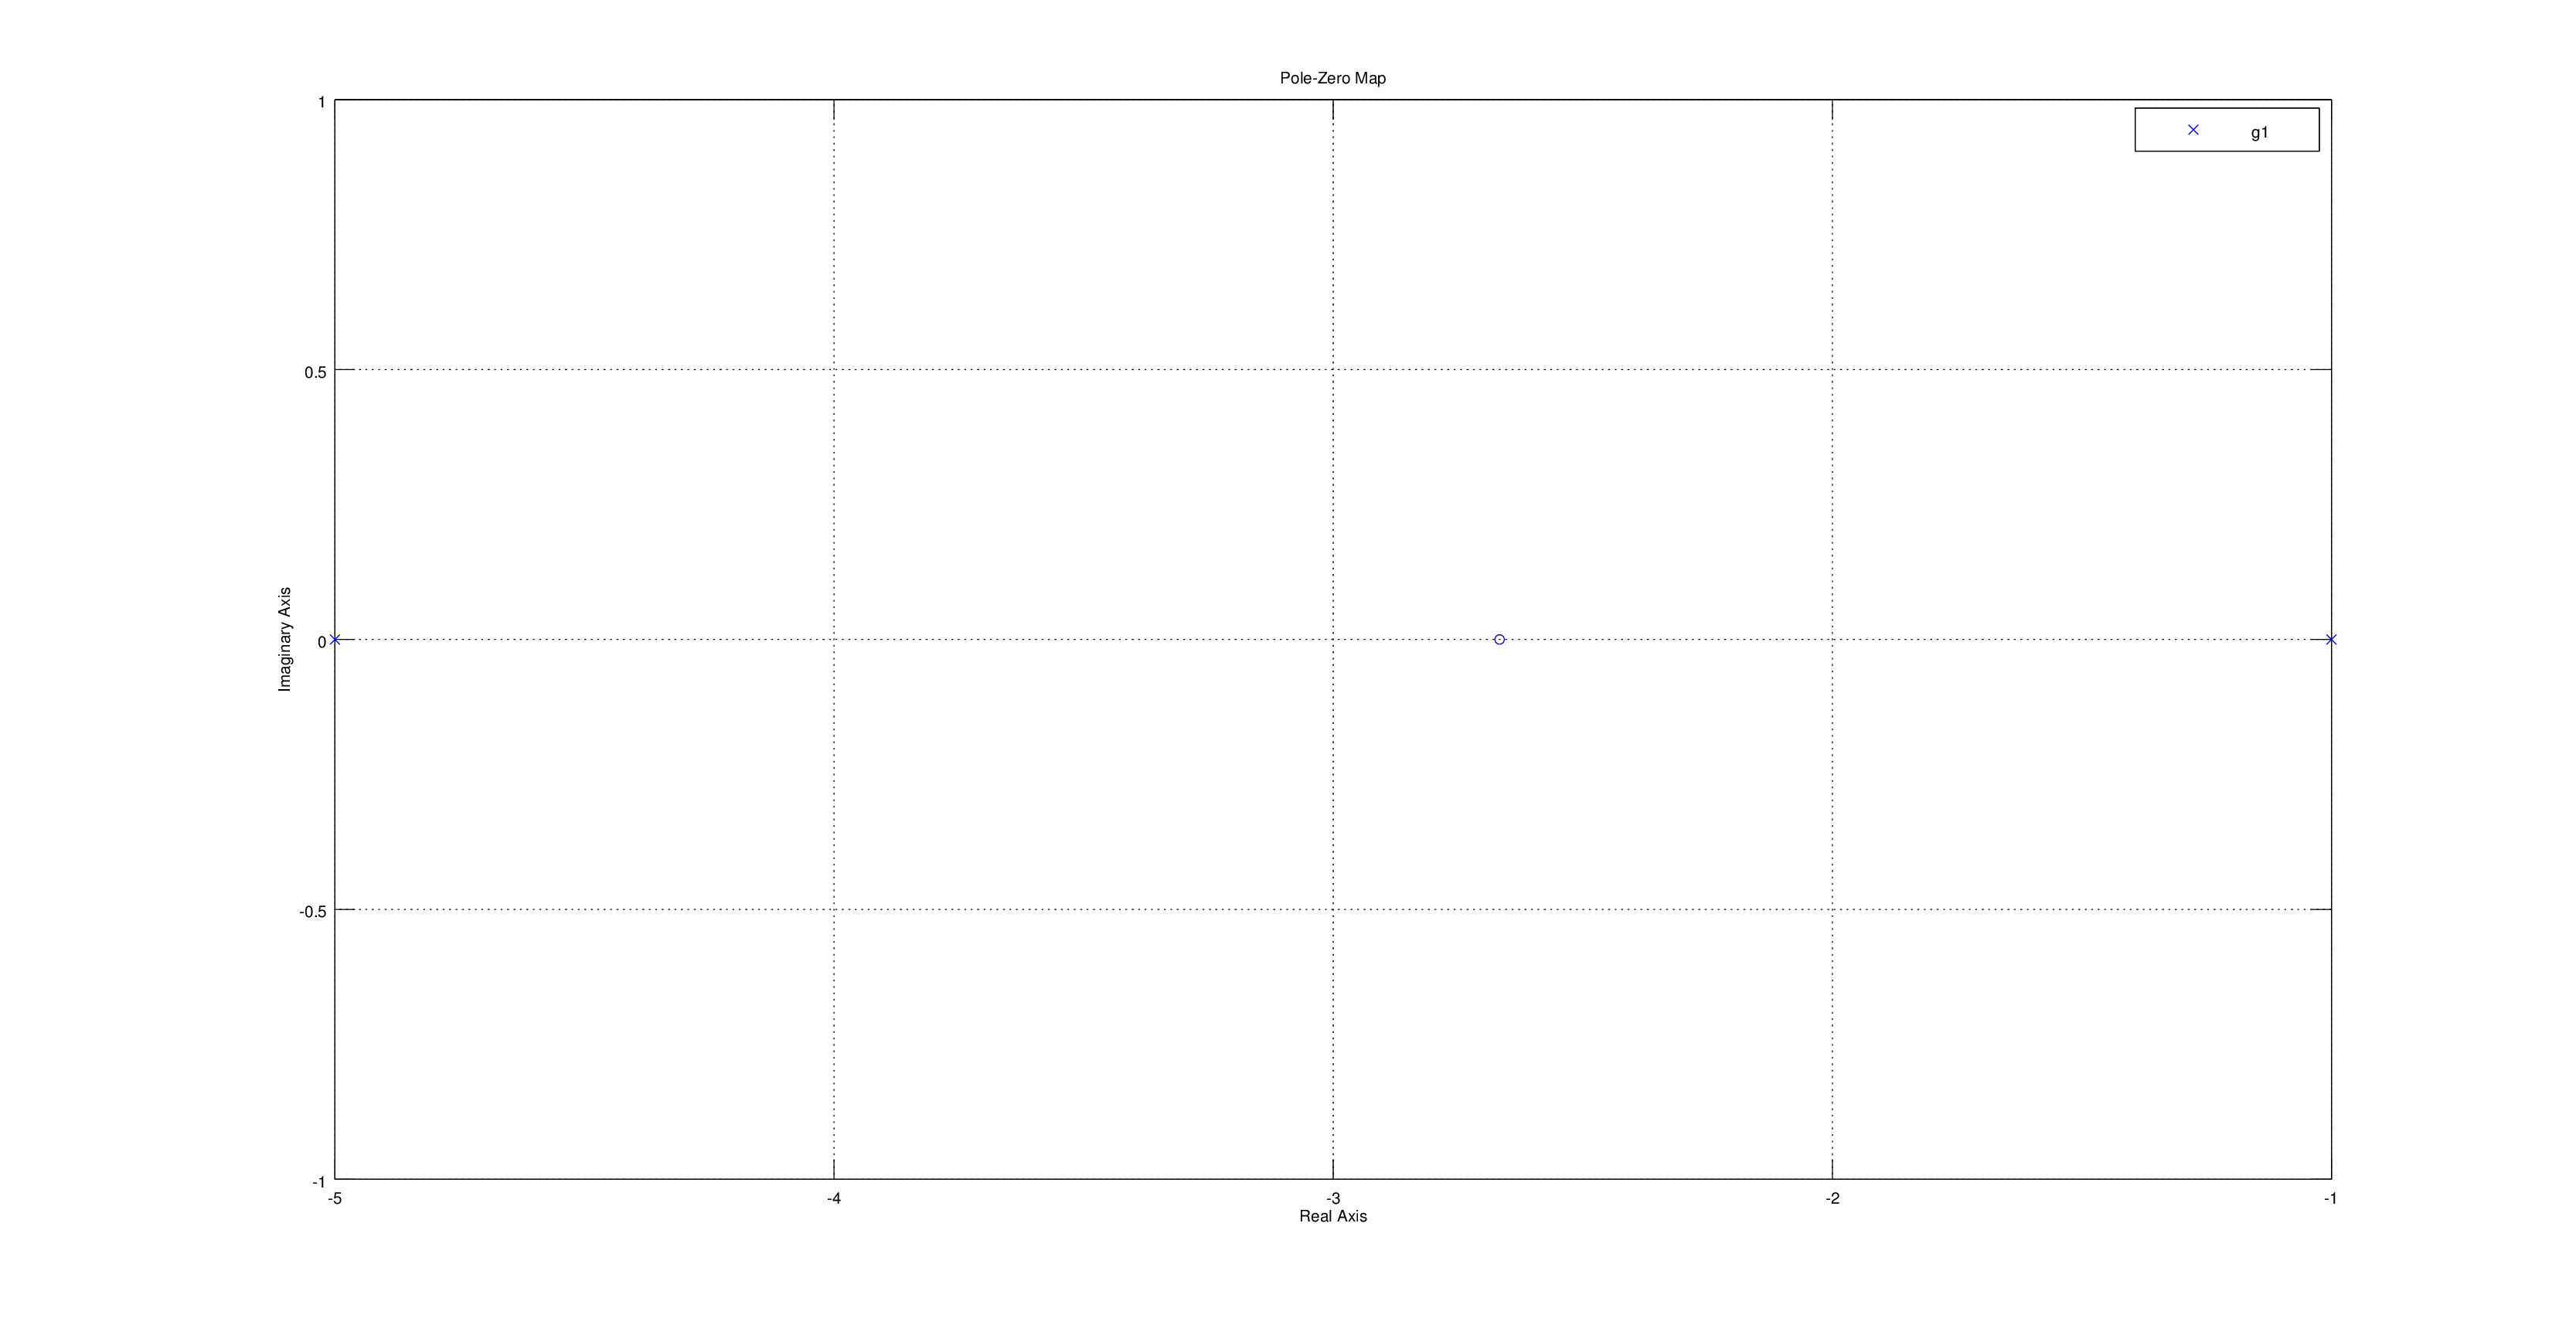
\includegraphics[width=\textwidth]{g1.png}
	\caption{$\mathrm{G}_1$ Pole-Zero Graph}
\end{figure}
\begin{figure}[H]
	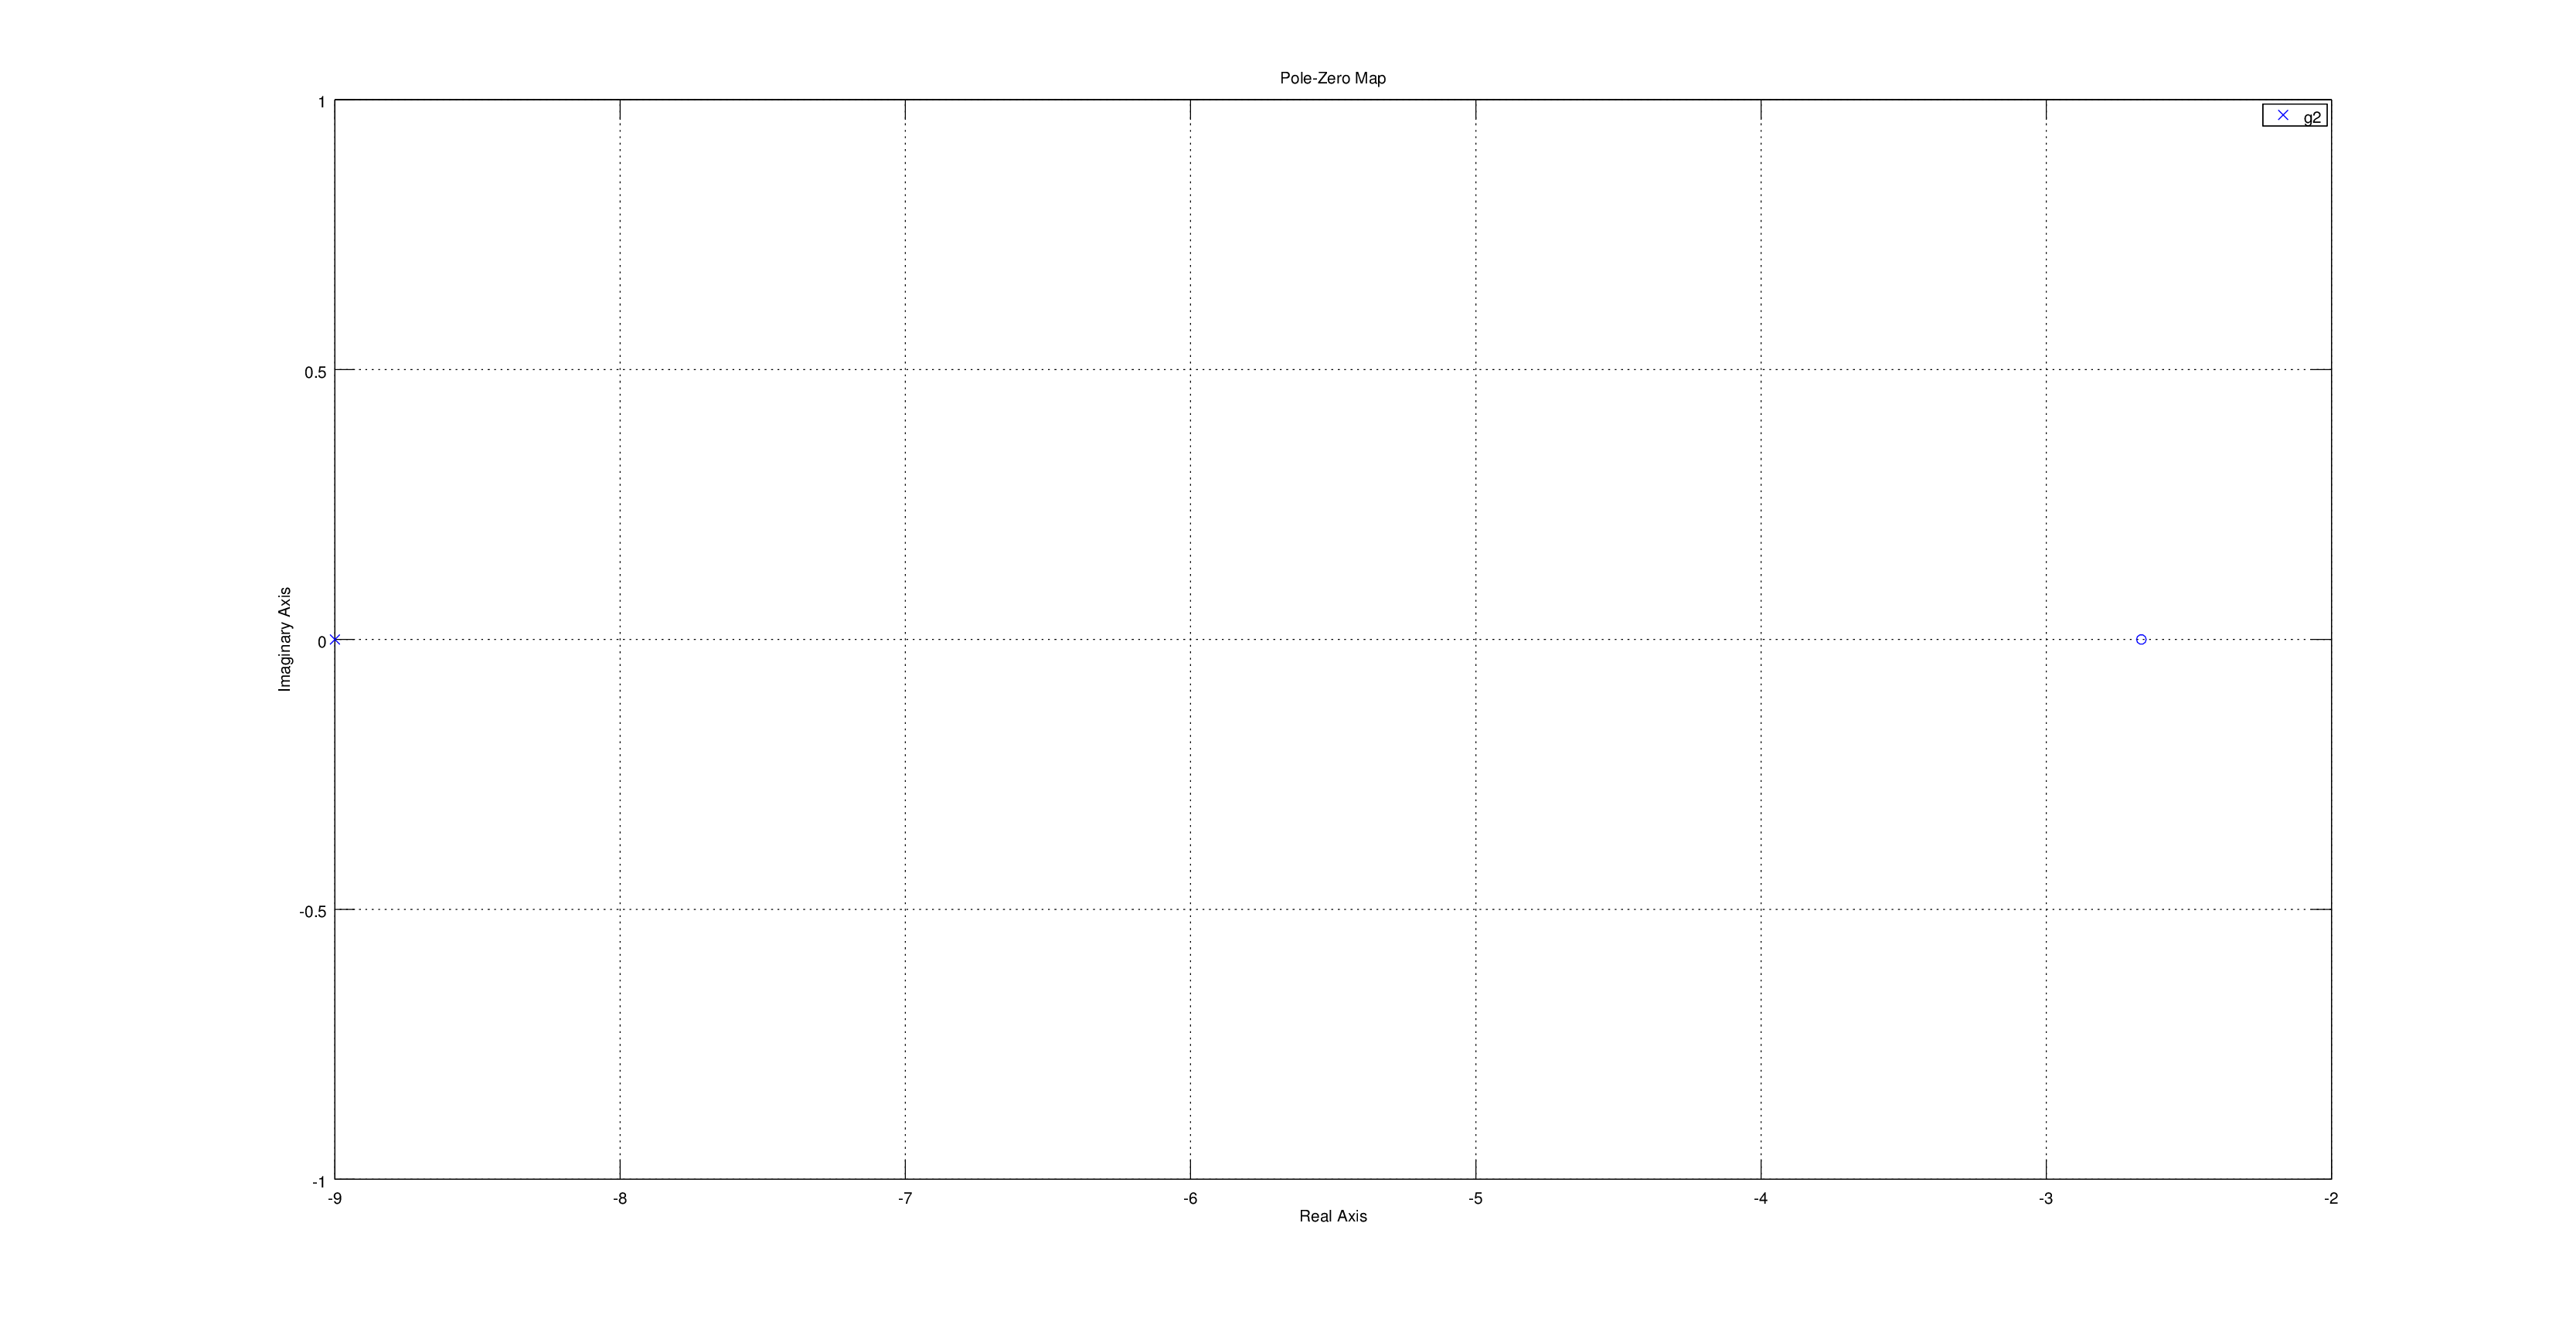
\includegraphics[width=\textwidth]{g2.png}
	\caption{$\mathrm{G}_2$ Pole-Zero Graph}
\end{figure}

\begin{figure}[H]
	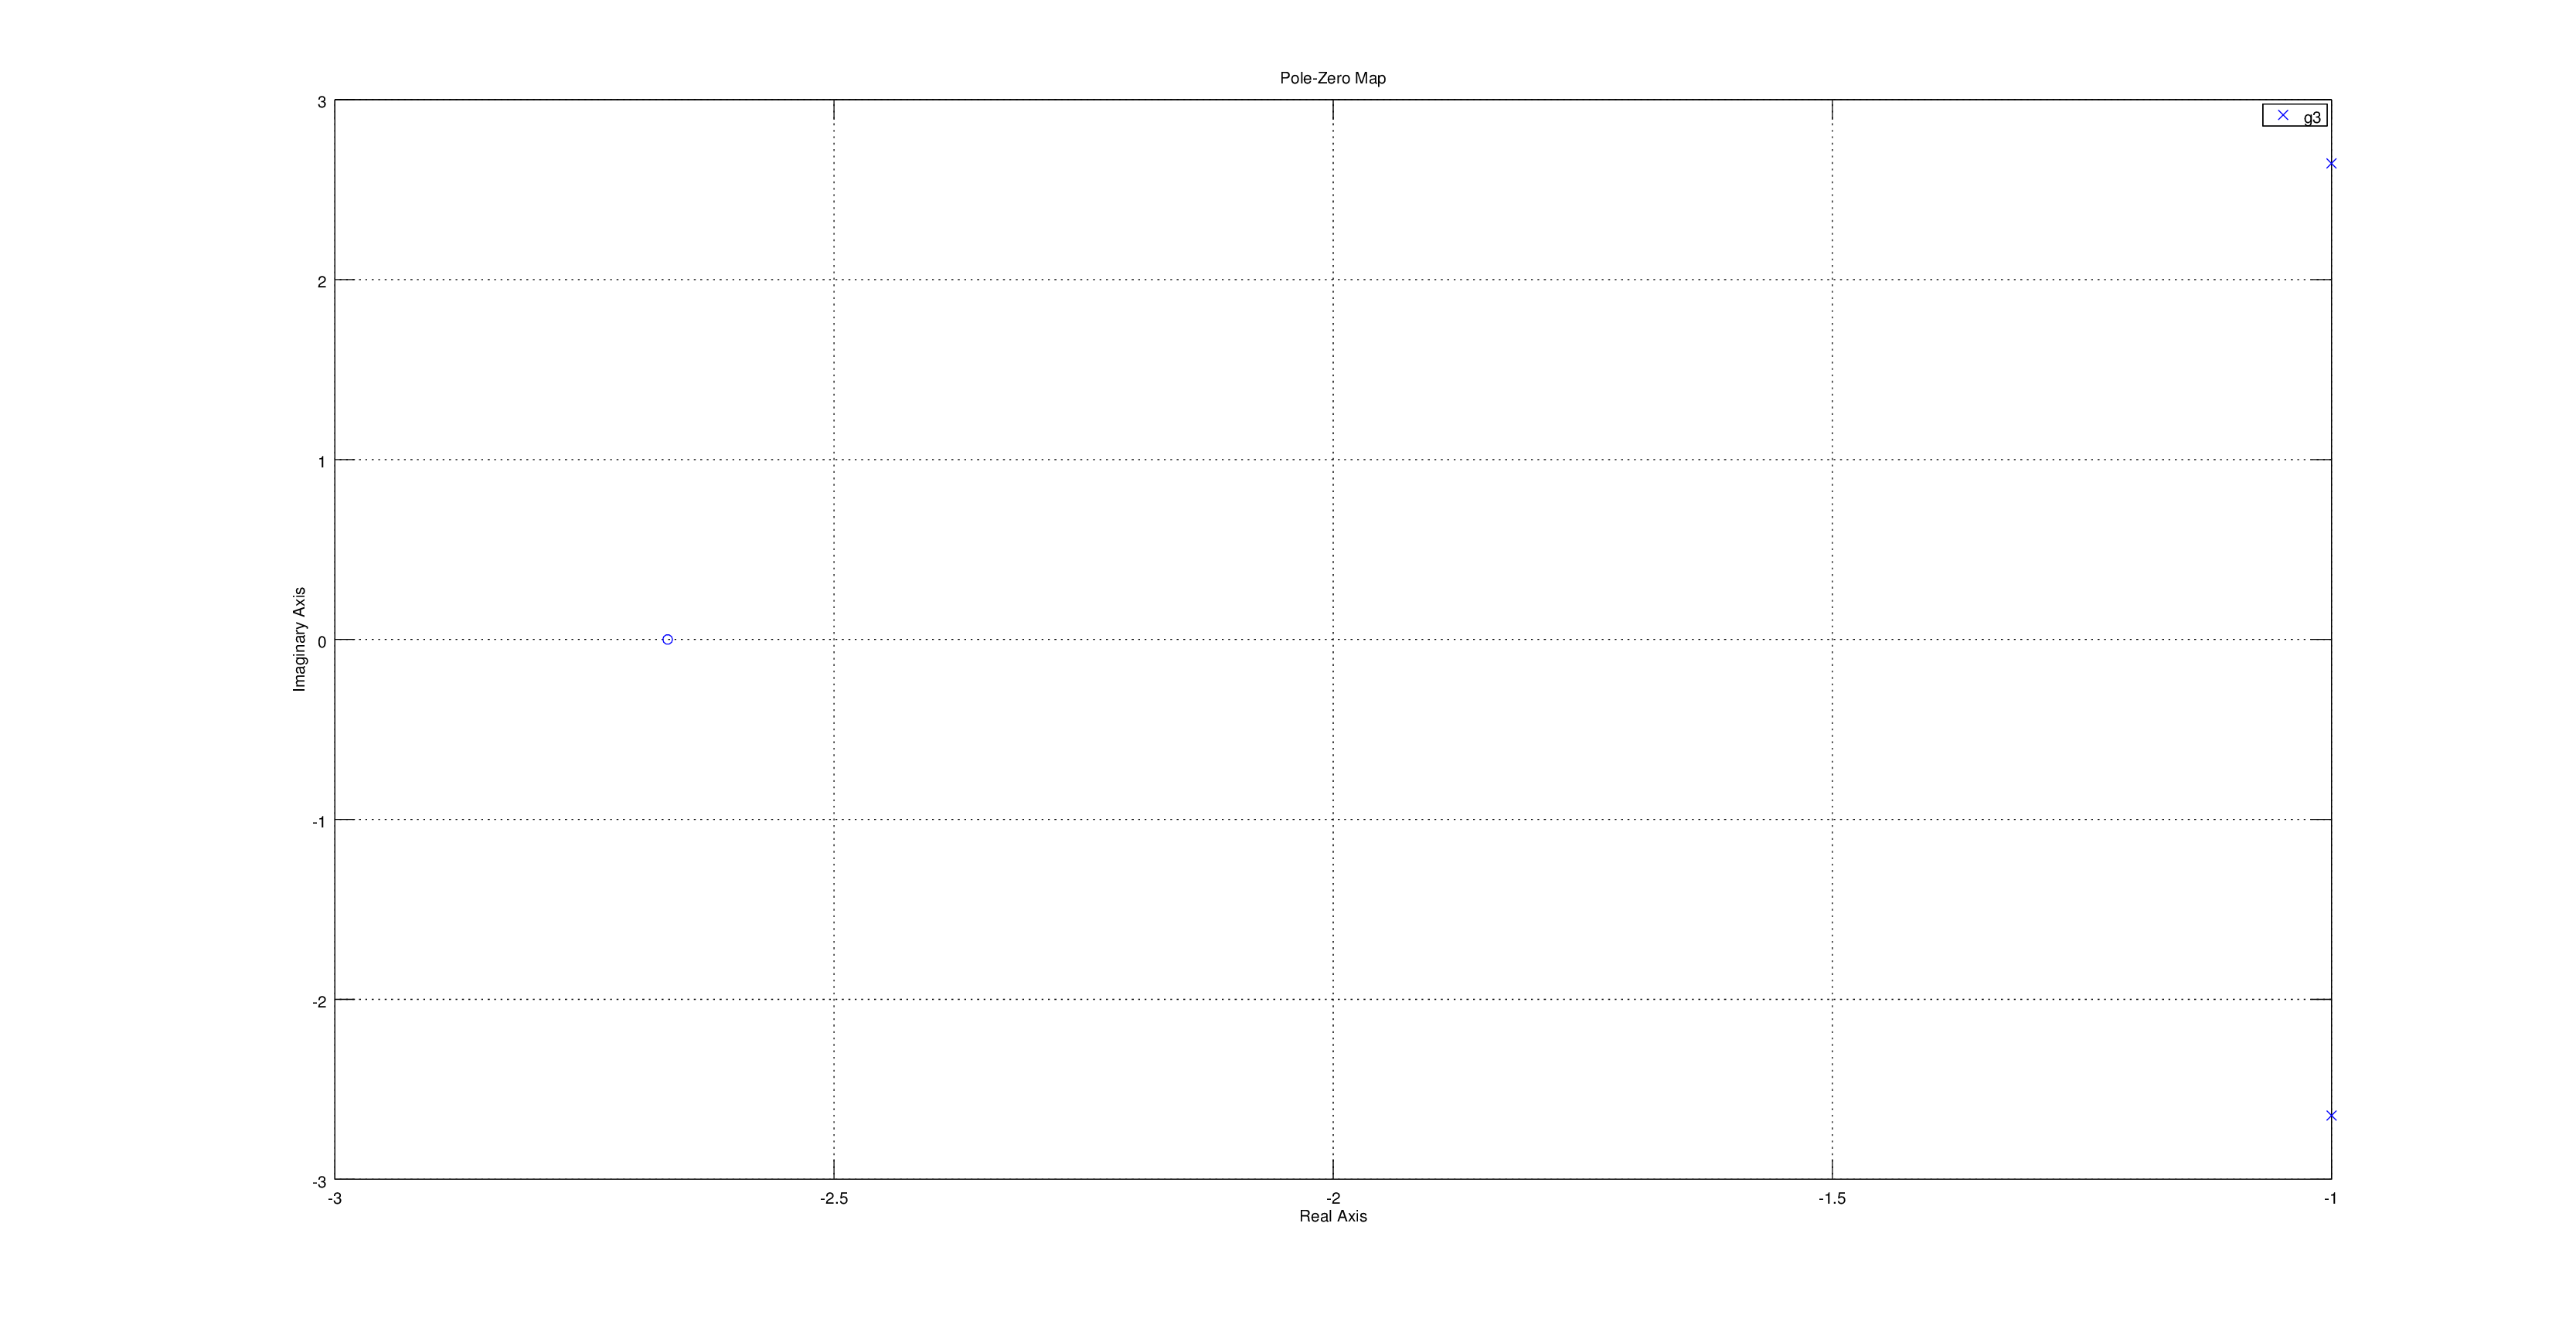
\includegraphics[width=\textwidth]{g3.png}
	\caption{$\mathrm{G}_3$ Pole-Zero Graph}
\end{figure}

\begin{figure}[H]
	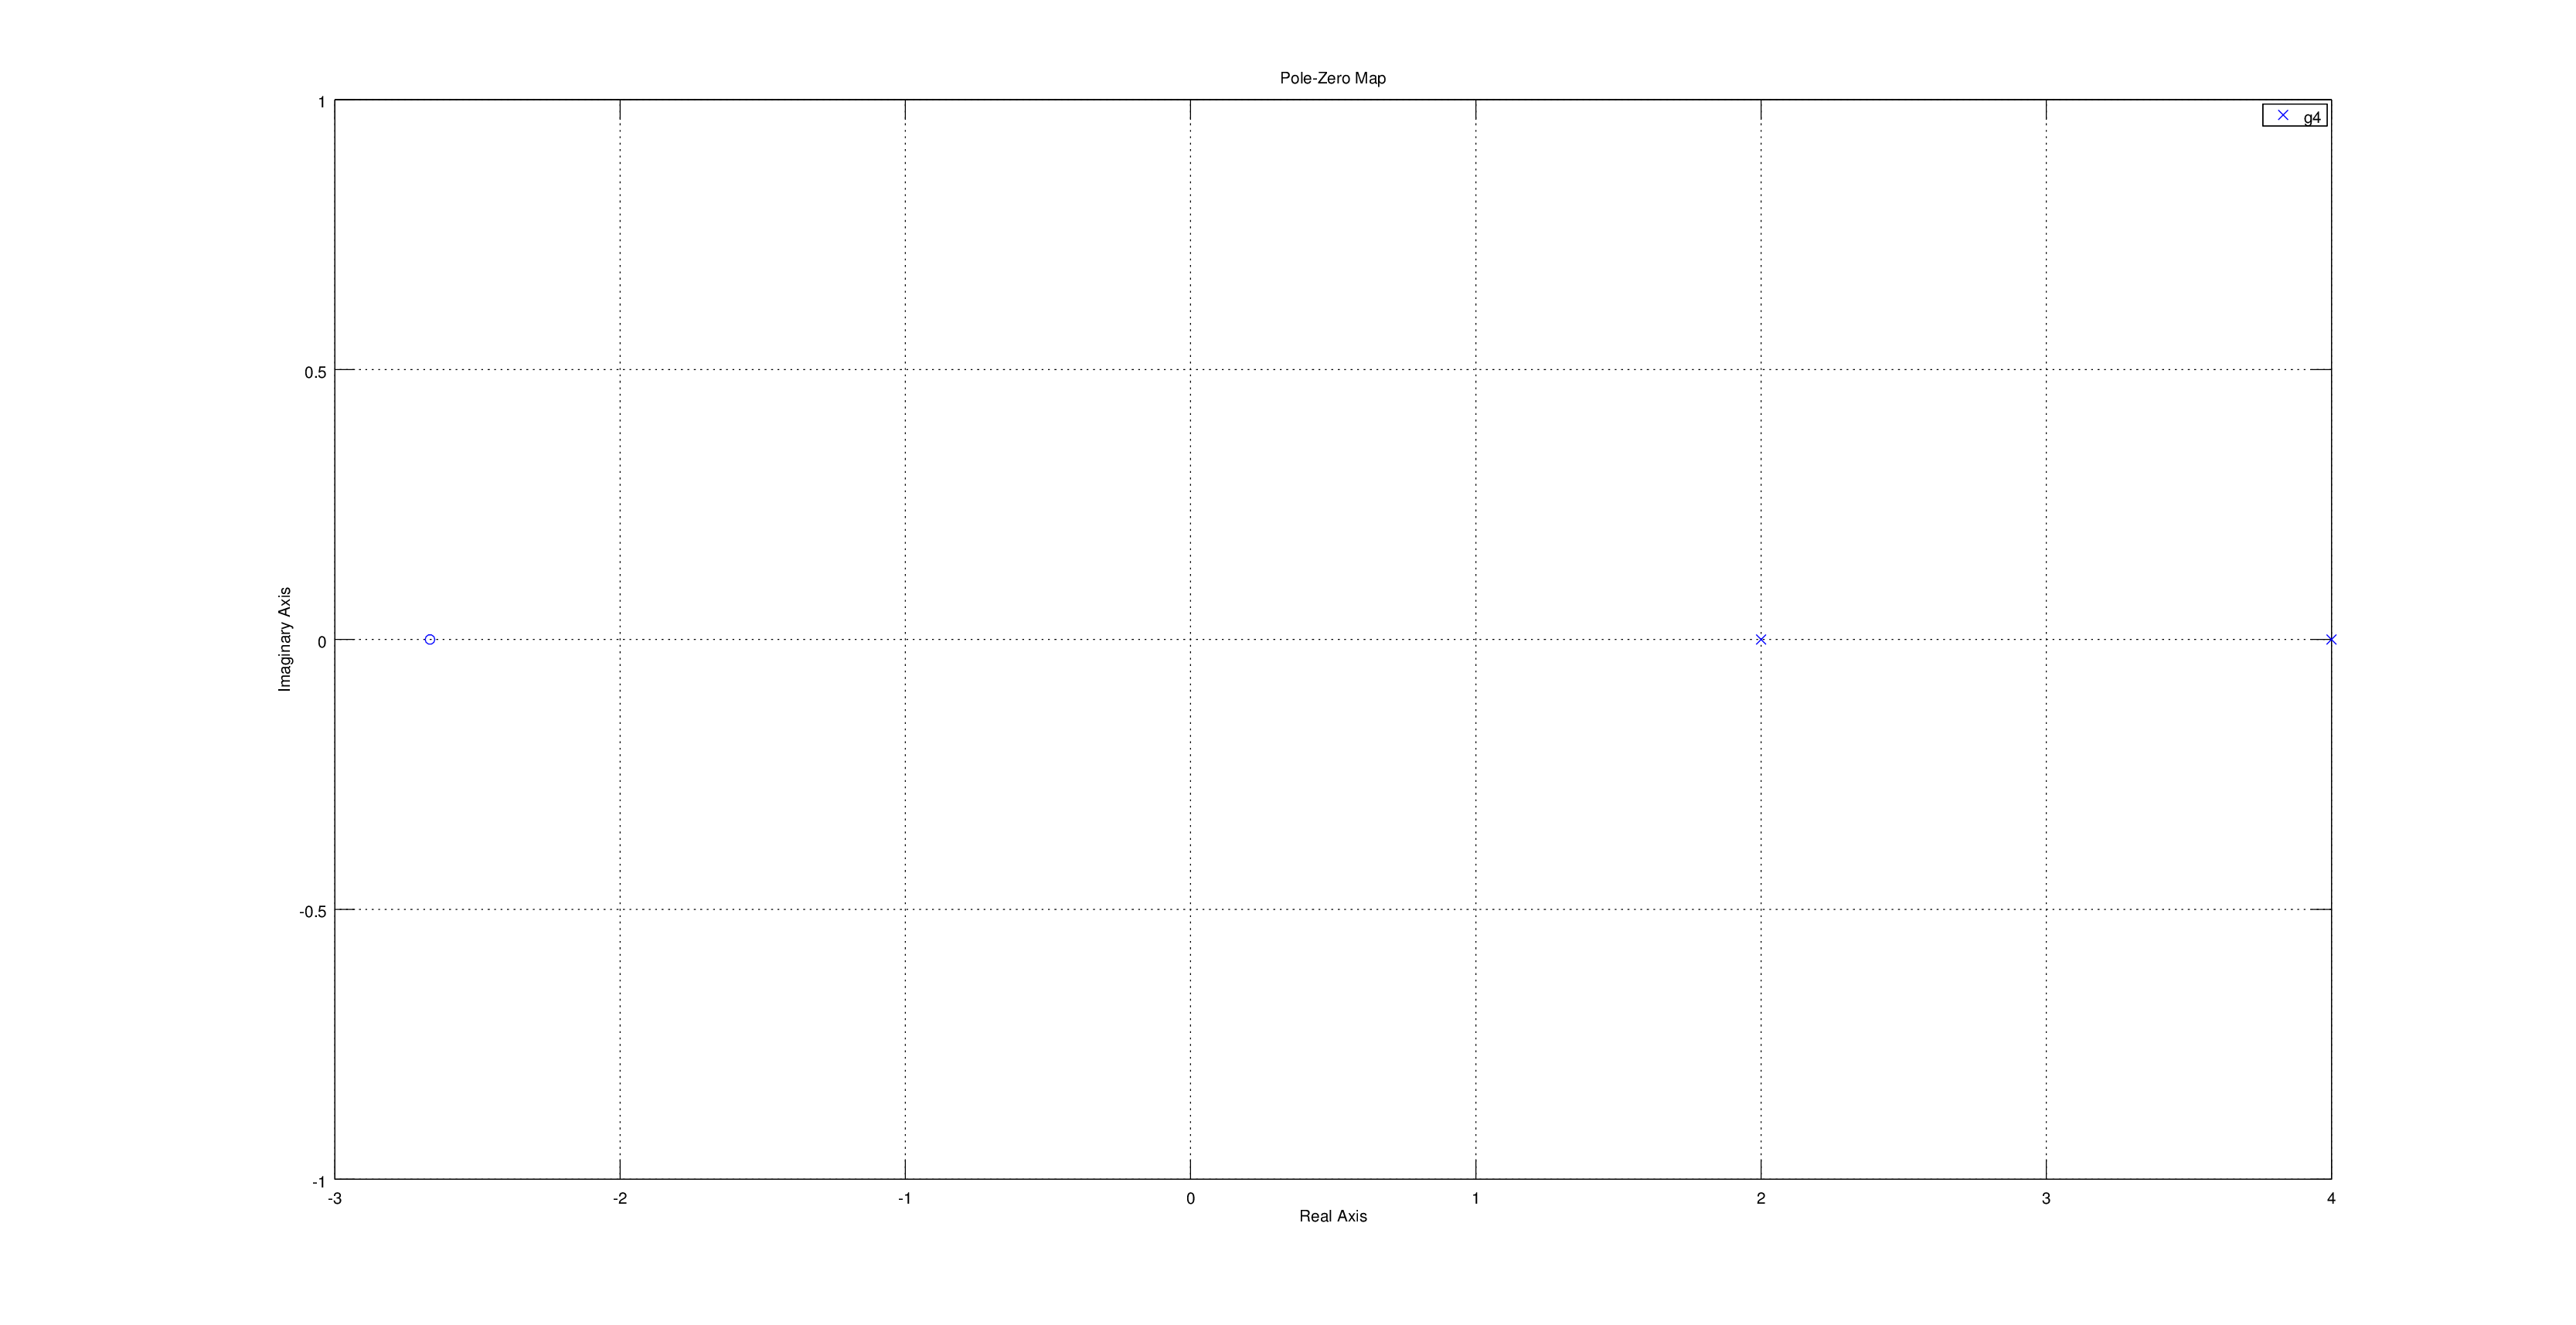
\includegraphics[width=\textwidth]{g4.png}
	\caption{$\mathrm{G}_4$ Pole-Zero Graph}
\end{figure}


% section graphs (end)


\section{Source Code} 
\label{sec:source_code}

\lstinputlisting[language=octave,title=lab1.m]{src/main.m}


% section source_code (end)
